\documentclass[a4paper]{exam}
\usepackage[export]{adjustbox}
\usepackage{geometry}
\usepackage{graphicx}
\usepackage{hyperref}
\usepackage{pythonhighlight}
\usepackage{tabularx}


\printanswers

\title{Homework Assignment 1}
\author{CS/CE 412/471 Algorithms: Design and Analysis}
\date{Spring 2025}

% \qformat{{\large\bf \thequestion. \thequestiontitle}\hfill}
\boxedpoints

\begin{document}
\maketitle
\thispagestyle{empty}


\includegraphics[trim=0 5cm 0 1cm, clip, width=\textwidth]{title}
\begin{questions}
  
\question[5]
  Sort the order of growth of the following 8 functions and justify your solution.
  \[
    7n,\; \lg n^{\lg n},\; n^{\lg n},\; n^2\lg n,\; \left(\frac{n}{2}\right)^{\frac{n}{2}},\; 3^{n^3},\; n^{\lg 3},\; n^2
  \]
  If some have the same asymptotic growth, then be sure to indicate that. As usual, $\lg$ indicates a base of 2.
    \begin{solution}
      
    \end{solution}

\question
  Prove or disprove each of the following:
  \begin{parts}
  \part[5] $f(n) = \Theta\left( f\left(\frac{n}{4}\right)\right)$
    \begin{solution}
      
    \end{solution}
  \part[5] $2^n = o(2^{\frac{n}{2}})$ (i.e. $2^n = O(2^{\frac{n}{2}})$ and $2^n \ne \Theta(2^{\frac{n}{2}})$
    \begin{solution}
      
    \end{solution}
  \part[5] $\Theta(f(n)) + \Theta(g(n))=\Theta(f(n)+g(n))$
    \begin{solution}
      
    \end{solution}
  \end{parts}
% \question
% Let $L$ be an array $L[1:n]$. The number of inversions in $L$ is the number of pairs $i < j$ such that $L[i] > L[j]$. Prove or disprove that counting the number of inversions requires at least $\Theta(n \lg n)$ comparisons in the worst case.

\question You are given 2 problems below. You need to design an efficient algorithm for each of them. Specifically,
    \begin{enumerate}
    \renewcommand{\theenumi}{\roman{enumi}} % Set enumeration to a, b, c...
    \item Clearly state the problem. For example, see how the sorting problem is stated on the first page of Chapter 1 of CLRS.
    \item Describe your algorithm. Follow the pseudocode conventions listed in Section 2.1 of CLRS. \textit{Do not} use programming language features, e.g. \pyth{list.append().}
    \item Illustrate, in any suitable manner, a run of your algorithm on a sample input.
    \item Describe the best and worst case for your algorithm.
    \item Describe an input, if any, on which your algorithm may not work correctly.
    \item Provide a time complexity analysis of your algorithm in terms of input size $n$ using asymptotic notation.
    \end{enumerate}

  \begin{parts}
  \part[5] Given a number, $x$, and an array, $A$, containing $n$ numbers, decide if the array contains two numbers $a$ and $b$ such that $a+b = x$.
    \begin{solution}
      
    \end{solution}
  \part[5] Given $k$ sorted lists containing a total of $n$ numbers, combine them to create a single sorted list of the $n$ numbers.
    \begin{solution}
      
    \end{solution}
  \end{parts}
  
\question For each of the following recurrences, derive a solution to the recurrence (show your working) and compare your solution with that obtained through the master theorem (show how it applies). 
  \begin{parts}
  \part[5] $T(n) = 2T\left(\frac{n}{4}\right) + 1$
    \begin{solution}
      
    \end{solution}
  \part[5] $T(n) = 2T\left(\frac{n}{4}\right) + n$
    \begin{solution}
      
    \end{solution}
  \part[5] $T(n) = 2T\left(\frac{n}{4}\right) + n^2$
    \begin{solution}
      
    \end{solution}
  \end{parts}


\question[5]\ 
  
  \begin{tabularx}{\textwidth}{c|X}
    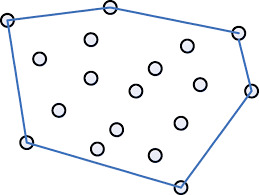
\includegraphics[scale=0.3,valign=t]{hull}
      &
  The \textit{convex hull} of a set of 2D points is a subset of the points that forms a \href{https://en.wikipedia.org/wiki/Convex_polygon}{convex polygon} which contains all the other points. It can be described informally as, the shape enclosed by a rubber band stretched around the points. 
  \end{tabularx}
  \begin{parts}
  \part[5] Design a divide and conquer algorithm to compute the convex hull of a set of 2D points and describe it using the pseudocode conventions listed in Section 2.1 of CLRS.
    \begin{solution}
      
    \end{solution}
  \part[5] Visualize the running of your algorithm as an \href{https://matplotlib.org/stable/users/explain/animations/animations.html}{animation} and submit the animation as an MP4 file.
  \end{parts}
  
\end{questions}

\end{document}

%%% Local Variables:
%%% mode: latex
%%% TeX-master: t
%%% End:
